\subsubsection{Placa de prototipagem eletrônica Arduino}

% SLIDE DE PLACA DE PROTOTIPAGEM ELETRÔNICA ARDUINO
\begin{frame}
\frametitle{Placa de prototipagem eletrônica Arduino}

Funções:

O sistemas de transmissão de potência será dado por meio de fuso trapezoidal. 
O fuso terá as seguintes características:

\begin{itemize}
    \item Recepção e tratamento dos dados provenientes da interface computacional;
    \item O controle dos motores está fundamentado na programação do microcontrolador de acordo com as necessidades definidas inicialmente para operação da mesa cartesiana.
\end{itemize}

\end{frame}
    
% SLIDE DE PLACA DE PROTOTIPAGEM ELETRÔNICA ARDUINO
\begin{frame}
\frametitle{Placa de prototipagem eletrônica Arduino}

\begin{figure}
\centering
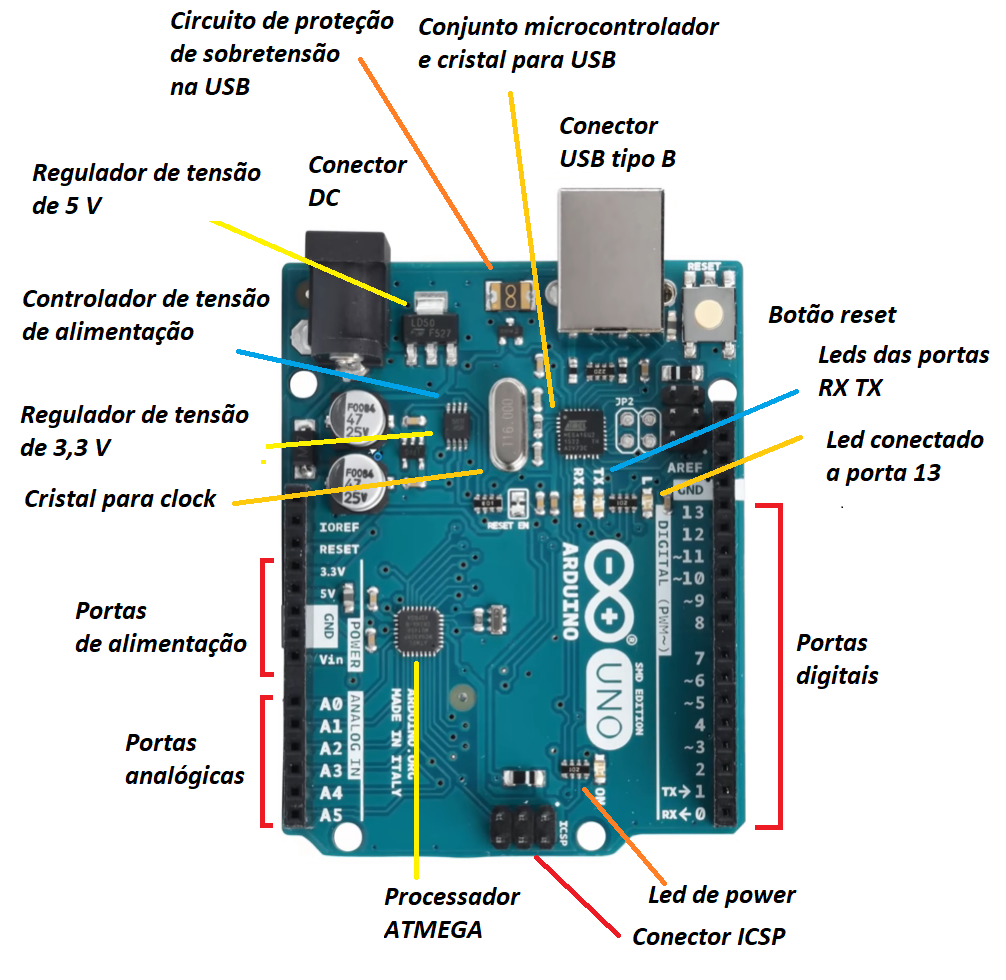
\includegraphics[scale = 0.3]{figs/placaarduino}
\end{figure}

\end{frame}
